\documentclass[titlepage]{article}
\usepackage[parfill]{parskip}
\usepackage[utf8]{inputenc}
\usepackage{float}
\usepackage{graphicx}
\graphicspath{ {./graphs/} }

\title{Computer Science 2XC3 Lab 4/5}
\author{Gregory Archer, Will Clubine, Gaurav Sharma}
\date{February 8th 2023}

\begin{document}

\maketitle
\tableofcontents
\listoffigures

\newpage

\section{Executive Summary}
\begin{itemize}
    \item Experiment 1 showed that
    \item Experiment 2 showed that
\end{itemize}

\section{Part 1}

\subsection{Experiment 1}

Experiment 1 examines the probability of a graph containing cycles as the proportion of edges to nodes increases.

The probability of a graph containing a cycle was computed by generating 500 random graphs with a given number of edges and nodes, and observing how many were cyclical.

We completed this process for graphs containing 5, 10, 15 and 20 nodes, with the proportion of edges varying from 0\% to 120\%, in increments of 20\%.

The result was then graphed in Figure 1 below.

\begin{figure}[H]
    \centering
    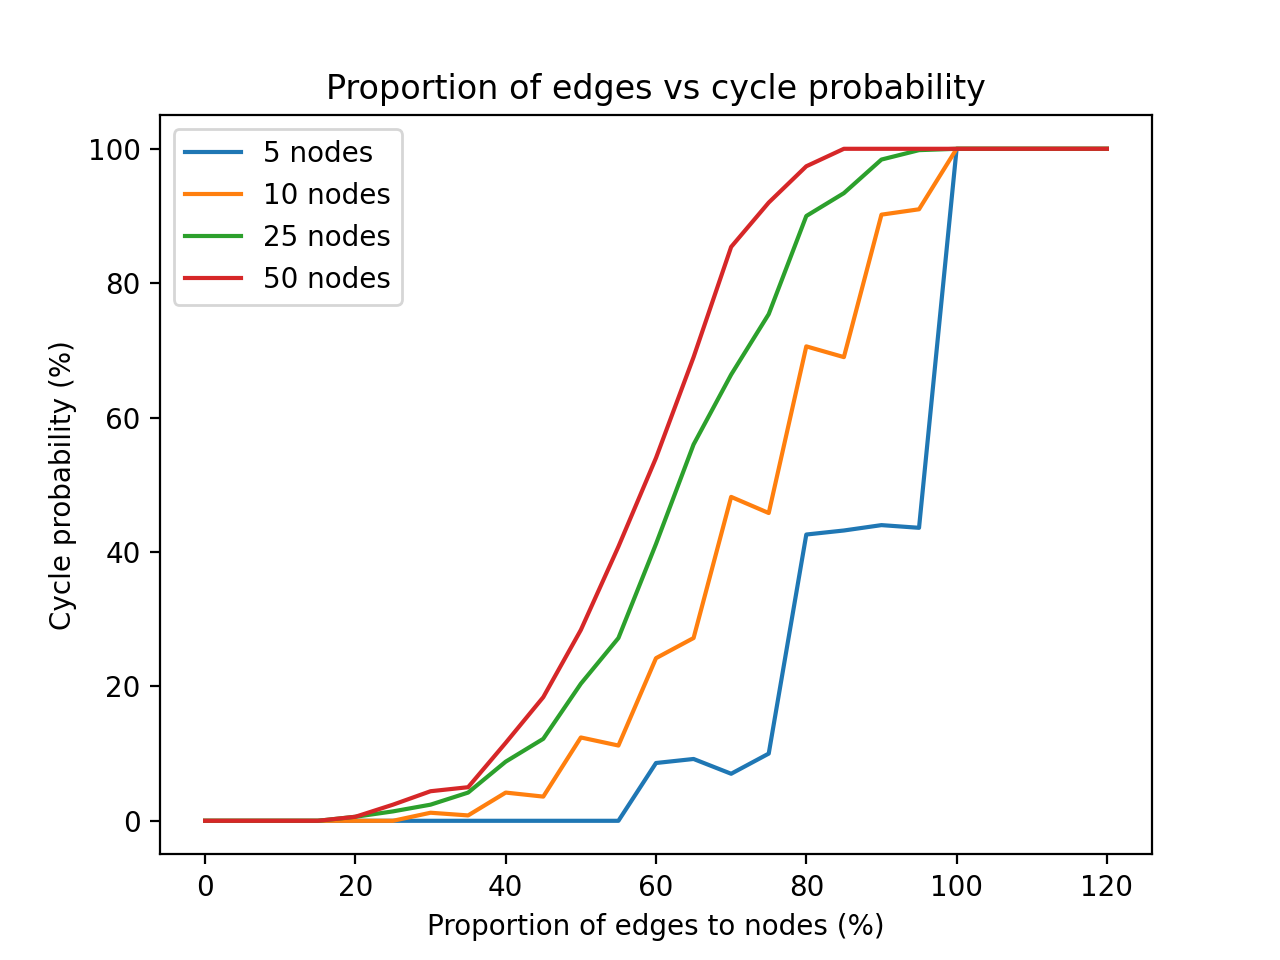
\includegraphics[width=0.8\linewidth]{experiment_1.png}
    \caption{Proportion of edges vs cycle probability}
    \label{fig:edges_vs_cycle}
\end{figure}

We have concluded from our results that as the proportion of edges relative to the number of nodes increases, the cyclical probability grows, showing a direct correlation. As the number of nodes increases, the probability of a graph containing a cycle - with the same relative proportions - increases, showing another direct correlation

Additionally, once the proportion of edges to nodes is 100\%, there will always be a cycle in the graph, regardless of the number of nodes. This is expected as any graph with equal or more edges than nodes must contain a cycle.

\subsection{Experiment 2}

Experiment 2 examines the probability of a graph being connected as the proportion of edges to nodes increases.

We compute the approximate connected probability for a graph of $e$ edges and $n$ nodes by generating 500 random graphs with $e$ edges and $n$ nodes and determining what percentage of those graphs are connected.

This process is conducted for graphs with 5, 10, 25, and 50 nodes at different proportions of edges. Specifically, we start with 0 edges and gradually increase to 500\% the node count in 20\% increments. The result is then graphed as shown in Figure \ref{fig:edges_vs_connected} below.

\begin{figure}[H]
    \centering
    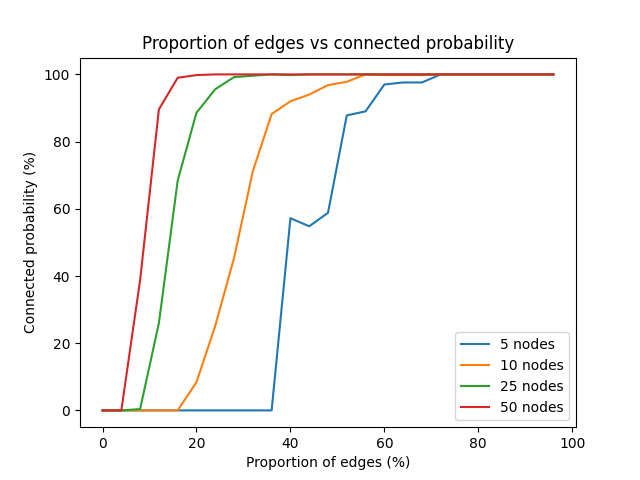
\includegraphics[width=0.8\linewidth]{experiment_2.png}
    \caption{Proportion of edges vs connected probability}
    \label{fig:edges_vs_connected}
\end{figure}

% this is wrong v will rewrite

As seen in Figure \ref{fig:edges_vs_connected}, each graph sits at a 0\% chance of connectedness before rapidly increasing and eventually reaching a 100\% probability of being connected. However, the proportion of edges at which the probability starts and stops rising increases with the number of nodes.

This is because the maximum number of unique edges --- and thus the number of ways the graph can be disconnected --- grows quadratically with the number of nodes. Specifically, a graph of $n$ nodes with no self-loops can have a maximum of $\Sigma_{i=0}^{n-1}i = \frac{(n - 1) \cdot n}{2}$ unique edges. This means a graph of 5 nodes has already reached it's maximum number of edges (10) by 200\%, while a graph of 50 nodes will not reach it's maximum number of edges (1225) until 2450\%.

\section{Part 2}

\subsection{Minimum Vertex Cover Approximation}

\subsubsection{Experiment 1}



\subsubsection{Experiment 2}



\subsubsection{Experiment 3}



\subsection{Maximum Independent Sets}

To determine the relationship between minimum vertex covers (MVC) and maximum independent sets (MIS), we compared their average size for graphs of 10 nodes with 0 to 45 edges; the maximum for a graph of 10 nodes. At each number of edges, we found the MVC and MIS for 250 graphs and calculated the average length of each, as well as the sum of the average lengths. The results were then graphed as shown in Figure \ref{fig:mvc_mis} below.

\begin{figure}[H]
    \centering
    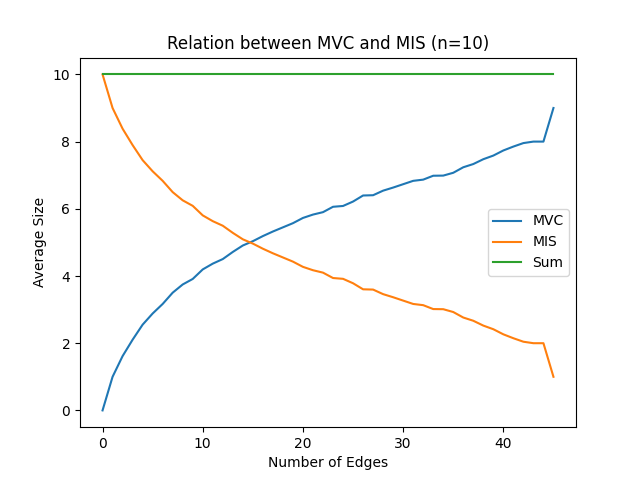
\includegraphics[width=0.8\linewidth]{mvc_mis.png}
    \caption{Relation between MVC and MIS}
    \label{fig:mvc_mis}
\end{figure}

As seen in Figure \ref{fig:mvc_mis}, the average MIS length decreased as the number of edges increased, while the average MVC length increased. Further, their sum was exactly equal to the number of nodes.

Looking closer, we can see that at 0 edges the MVC was empty while the MIS contained all nodes. This is expected because every node can be added to the MIS without connecting to another node, and there are no edge endpoints to be included in the MVC.

At the maximum number of edges, the MIS contains only one node while the MVC contains $n-1$ nodes. This is also expected, because the single node in the MIS connects to all other nodes, and the single node left out of the MVC has every edge taken care of by a node it is connected to.

These three observations leads us to the conclusion that the MVC of a graph is the complement of the MIS.

\appendix
\section{Navigating the Code}

\begin{itemize}
    \item Each experiment in Part 1 can be found within it's own file titled \verb|experiment_#.py|
    \item Approximation experiments can be found within \verb|approximation_experiments.py|
    \item Maximum independent set experiments can be found within \verb|independent_sets.py|
    \item Additional graph functions were added to \verb|graph.py|
\end{itemize}

\end{document}
